\documentclass[12pt,tikz,border=8pt]{standalone}
\usepackage{libertine}
\usepackage{amsmath,amssymb}
\usepackage{tikz}
\usetikzlibrary{arrows.meta,decorations.markings}

\begin{document}
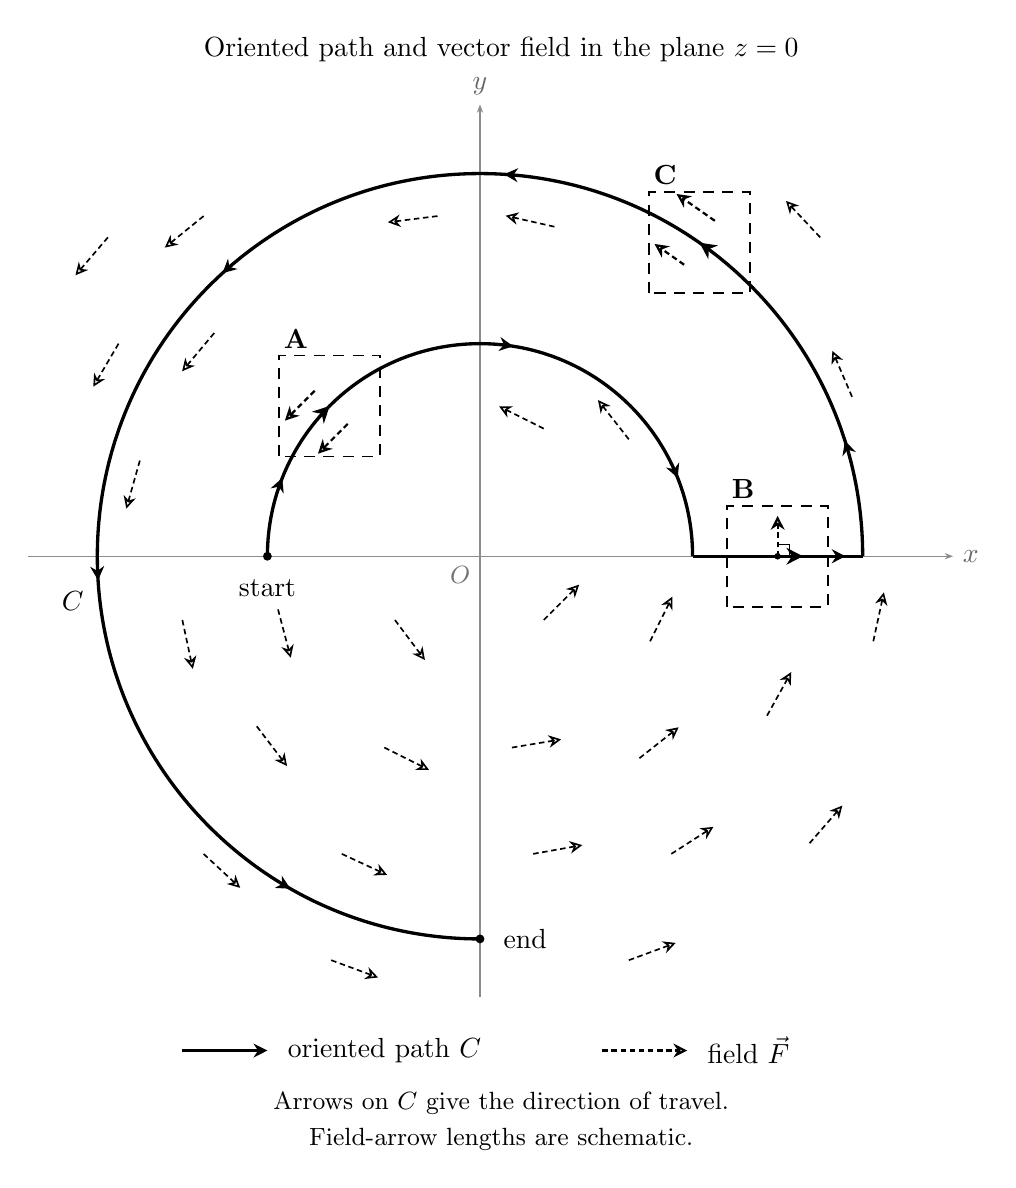
\begin{tikzpicture}[x=1.35cm,y=1.35cm,
  every node/.style={font=\normalsize},
  field/.style={black,dash pattern=on 2pt off 1.3pt,line width=0.6pt,
    -{Stealth[open,length=4.5pt,width=4.5pt]}},
  localfield/.style={field,line width=0.8pt,
    -{Stealth[open,length=5pt,width=5pt]}},
  curve/.style={black,line width=1.2pt},
  neighborhood/.style={black,dash pattern=on 4pt off 3pt,line width=0.65pt},
  axis/.style={black!45,line width=0.4pt,-{Stealth[length=3pt]}}]
  % Instructor construction (not displayed): F(x,y,0)=(-y,x,0).
  % The inner semicircle is clockwise; the radial connector is outward;
  % the outer three-quarter circle is counterclockwise.
  \def\ax{-1.4142135624}
  \def\ay{1.4142135624}
  \def\bx{2.8}
  \def\by{0}
  \def\cx{2.0648751709}
  \def\cy{2.9489473594}

  \draw[axis] (-4.25,0) -- (4.45,0) node[right,black!60] {$x$};
  \draw[axis] (0,-4.15) -- (0,4.25) node[above,black!60] {$y$};
  \node[below left,black!55,font=\small] at (0,0) {$O$};

  % Equal positive rescaling of each displayed field vector preserves its
  % direction. Omit samples near the highlighted comparisons and labels.
  \foreach \px/\py in {
    -3.5/3.0,-2.6/3.2,-0.4/3.2,0.7/3.1,3.2/3.0,
    -3.4/2.0,-2.5/2.1,0.6/1.2,1.4/1.1,3.5/1.5,
    -3.2/0.9,-2.8/-0.6,-1.9/-0.5,-0.8/-0.6,0.6/-0.6,1.6/-0.8,
    -2.1/-1.6,-0.9/-1.8,0.3/-1.8,1.5/-1.9,2.7/-1.5,
    -2.6/-2.8,-1.3/-2.8,0.5/-2.8,1.8/-2.8,3.1/-2.7,
    -1.4/-3.8,1.4/-3.8,3.7/-0.8}
  {
    \pgfmathsetmacro{\vl}{sqrt(\px*\px+\py*\py)}
    \draw[field] (\px,\py) -- ++({-0.47*\py/\vl},{0.47*\px/\vl});
  }

  % Distinct portions belong to one continuous, oriented path C.
  \draw[curve,postaction={decorate},decoration={markings,
    mark=at position 0.12 with {\arrow{Stealth[length=5pt,width=5pt]}},
    mark=at position 0.25 with {\arrow{Stealth[length=6pt,width=6pt]}},
    mark=at position 0.55 with {\arrow{Stealth[length=5pt,width=5pt]}},
    mark=at position 0.88 with {\arrow{Stealth[length=5pt,width=5pt]}}}]
    (-2,0) arc[start angle=180,end angle=0,radius=2];
  \draw[curve,postaction={decorate},decoration={markings,
    mark=at position 0.65 with {\arrow{Stealth[length=6pt,width=6pt]}},
    mark=at position 0.90 with {\arrow{Stealth[length=5pt,width=5pt]}}}]
    (2,0) -- (3.6,0);
  \draw[curve,postaction={decorate},decoration={markings,
    mark=at position 0.065 with {\arrow{Stealth[length=5pt,width=5pt]}},
    mark=at position 0.2037037037 with {\arrow{Stealth[length=6pt,width=6pt]}},
    mark=at position 0.32 with {\arrow{Stealth[length=5pt,width=5pt]}},
    mark=at position 0.49 with {\arrow{Stealth[length=5pt,width=5pt]}},
    mark=at position 0.68 with {\arrow{Stealth[length=5pt,width=5pt]}},
    mark=at position 0.89 with {\arrow{Stealth[length=5pt,width=5pt]}}}]
    (3.6,0) arc[start angle=0,end angle=270,radius=3.6];
  \fill (-2,0) circle[radius=1.6pt] node[below=5pt] {start};
  \fill (0,-3.6) circle[radius=1.6pt] node[right=5pt] {end};
  \node[fill=white,inner sep=2pt] at (-3.83,-0.42) {$C$};

  % Each square contains one smooth path segment. Filled arrowheads on the
  % curve give its orientation; no separate tangent vectors are drawn.
  \foreach \px/\py/\lab in {\ax/\ay/A,\bx/\by/B,\cx/\cy/C}
  {
    \draw[neighborhood] ({\px-0.475},{\py-0.475})
      rectangle ({\px+0.475},{\py+0.475});
    \node[anchor=south west,fill=white,inner sep=1.5pt,font=\bfseries]
      at ({\px-0.475},{\py+0.50}) {\lab};
  }
  % A: field arrows lie on either side of the path instead of overlapping
  % it. Positive radial shifts preserve the direction of F=(-y,x,0).
  \draw[localfield] ({1.10*\ax},{1.10*\ay}) -- ++(-0.28,-0.28);
  \draw[localfield] ({0.88*\ax},{0.88*\ay}) -- ++(-0.28,-0.28);
  % B: the field is vertical and perpendicular to the horizontal path.
  \draw[localfield] (\bx,\by) -- ++(0,0.38);
  \draw[black,line width=0.45pt]
    ({\bx+0.11},\by) -- ({\bx+0.11},{\by+0.11})
    -- (\bx,{\by+0.11});
  \fill (\bx,\by) circle[radius=1.2pt];
  % C: the field and the path point the same way. Radial offsets separate
  % the dashed field arrows from the solid path without changing directions.
  \draw[localfield] ({1.07*\cx},{1.07*\cy})
    -- ++({-0.44*sin(55)},{0.44*cos(55)});
  \draw[localfield] ({0.93*\cx},{0.93*\cy})
    -- ++({-0.34*sin(55)},{0.34*cos(55)});

  \node at (0.2,4.77) {Oriented path and vector field in the plane $z=0$};
  \draw[curve,-{Stealth[length=5pt,width=5pt]}] (-2.8,-4.65) -- (-2.0,-4.65);
  \node[right] at (-1.90,-4.65) {oriented path $C$};
  \draw[localfield] (1.15,-4.65) -- (1.95,-4.65);
  \node[right] at (2.05,-4.65) {field $\vec F$};
  \node[font=\small,align=center] at (0.2,-5.32) {
    Arrows on $C$ give the direction of travel.\\[2pt]
    Field-arrow lengths are schematic.
  };
\end{tikzpicture}
\end{document}
